% Generated by scripts/publish_workflow_results_to_thesis.py. Do not edit.
\begingroup
\setlength{\intextsep}{4pt}
\begin{figure}[htbp]
\centering
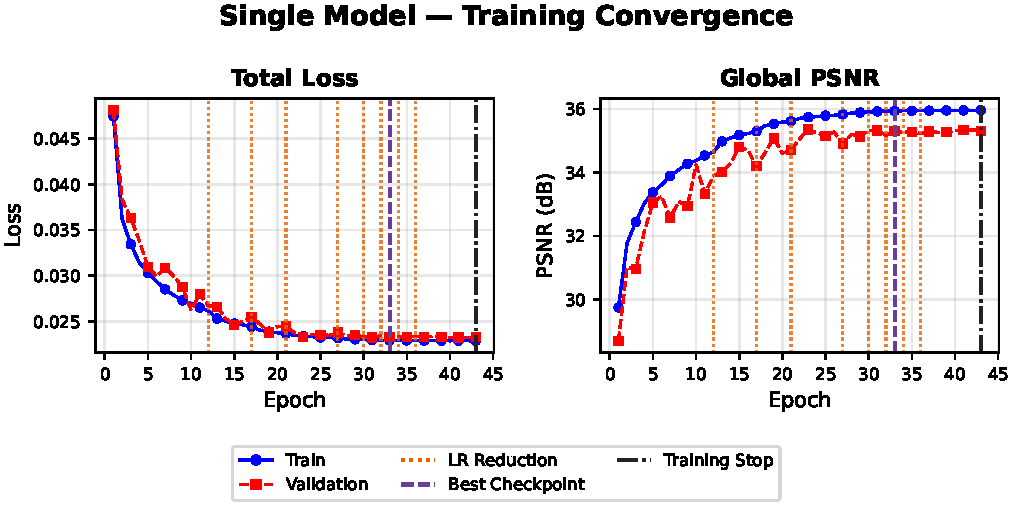
\includegraphics[width=0.98\linewidth]{Figures/Generated/training/training-curves-singlehead-pair-01-loss-psnr-6e359ebd.pdf}
\end{figure}

\begin{figure}[htbp]
\centering
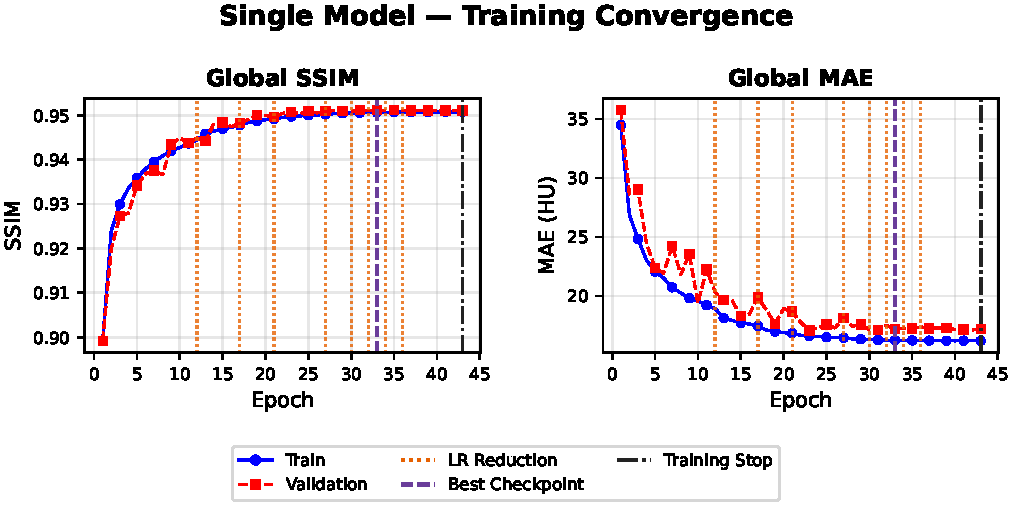
\includegraphics[width=0.98\linewidth]{Figures/Generated/training/training-curves-singlehead-pair-02-ssim-mae-80362d3f.pdf}
\end{figure}

\begin{figure}[htbp]
\centering
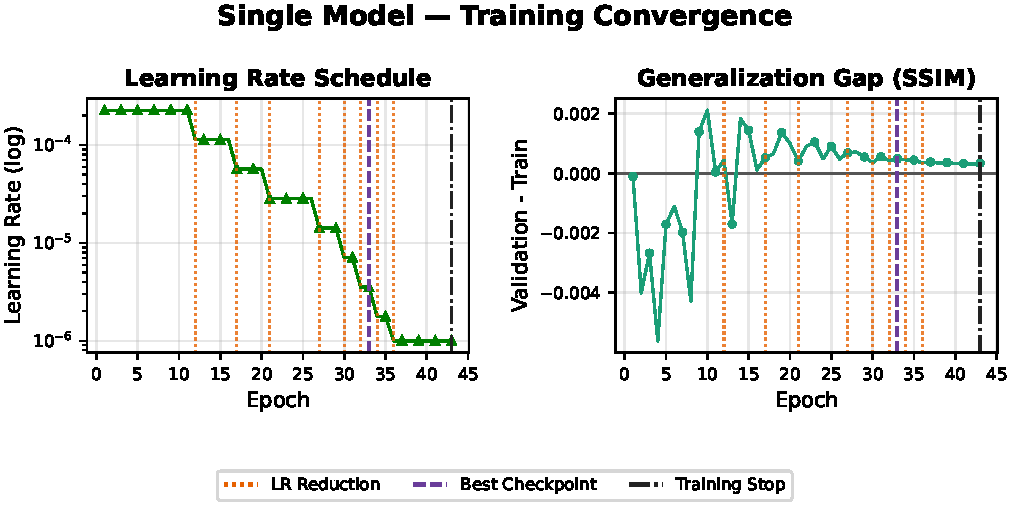
\includegraphics[width=0.98\linewidth]{Figures/Generated/training/training-curves-singlehead-pair-03-lr-gap-c975e425.pdf}
\end{figure}

\FloatBarrier
\captionsetup{skip=1.5pt}
\graphiccaptionof[Training convergence (results): Single Model, seed 2024]{Training convergence for the Single Model, seed 2024. Each chart pair repeats the shared legend so it remains interpretable if the group spans multiple pages. Orange dotted vertical lines indicate learning-rate reductions; the purple dashed line marks the epoch of the best validation checkpoint; and the black dash-dotted line marks training termination. The \textit{generalization-gap} panel reports validation minus training SSIM and supports inspection for persistent divergence compatible with overfitting.}
\label{fig:results-training-convergence-single-model-seed-2024}
\par\medskip
\endgroup

\begingroup
\setlength{\intextsep}{4pt}
\begin{figure}[htbp]
\centering
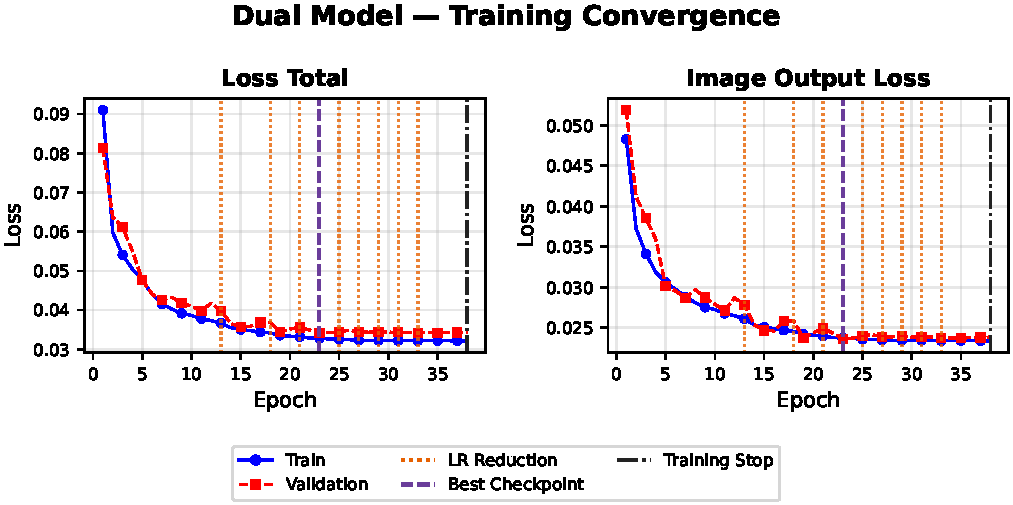
\includegraphics[width=0.98\linewidth]{Figures/Generated/training/training-curves-dualhead-pair-01-loss-419f6af3.pdf}
\end{figure}

\begin{figure}[htbp]
\centering
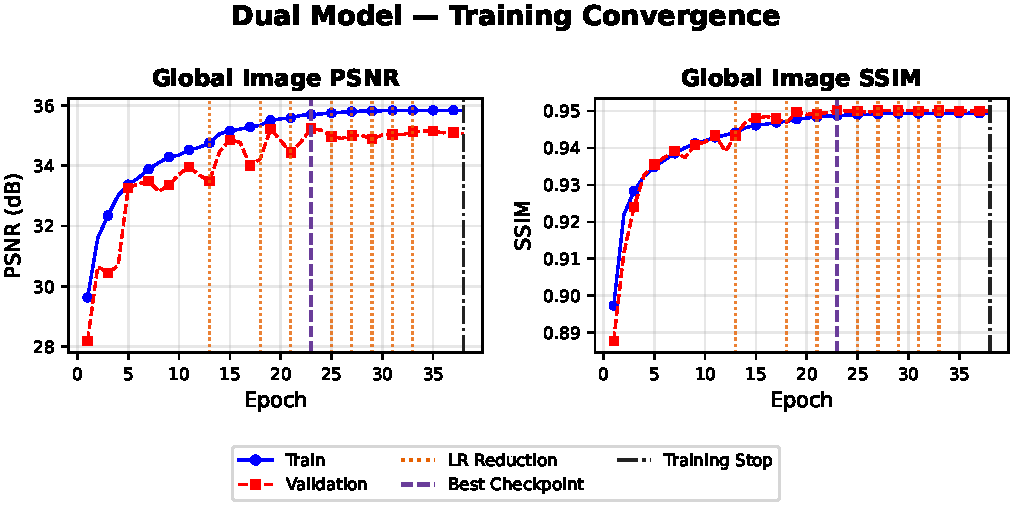
\includegraphics[width=0.98\linewidth]{Figures/Generated/training/training-curves-dualhead-pair-02-psnr-ssim-bc0a0156.pdf}
\end{figure}

\begin{figure}[htbp]
\centering
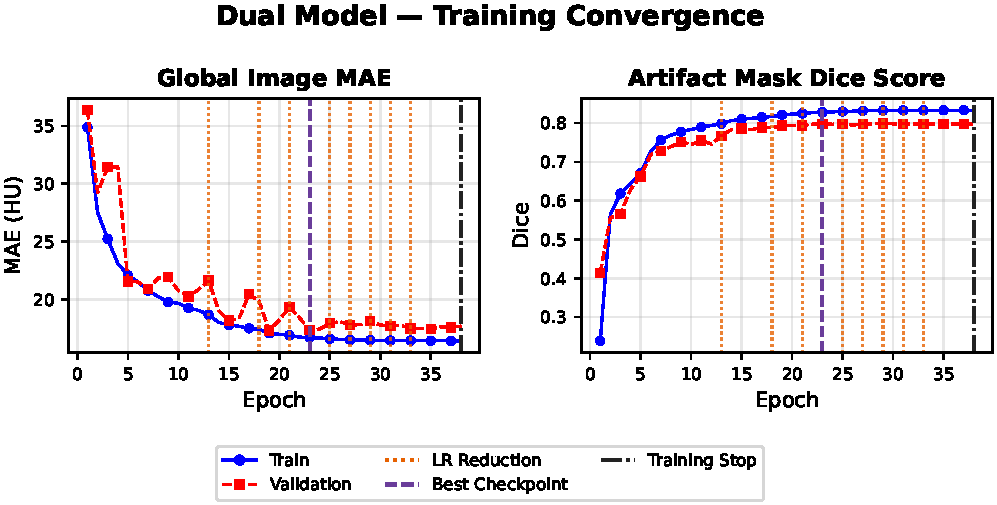
\includegraphics[width=0.98\linewidth]{Figures/Generated/training/training-curves-dualhead-pair-03-mae-dice-bde647ae.pdf}
\end{figure}

\begin{figure}[htbp]
\centering
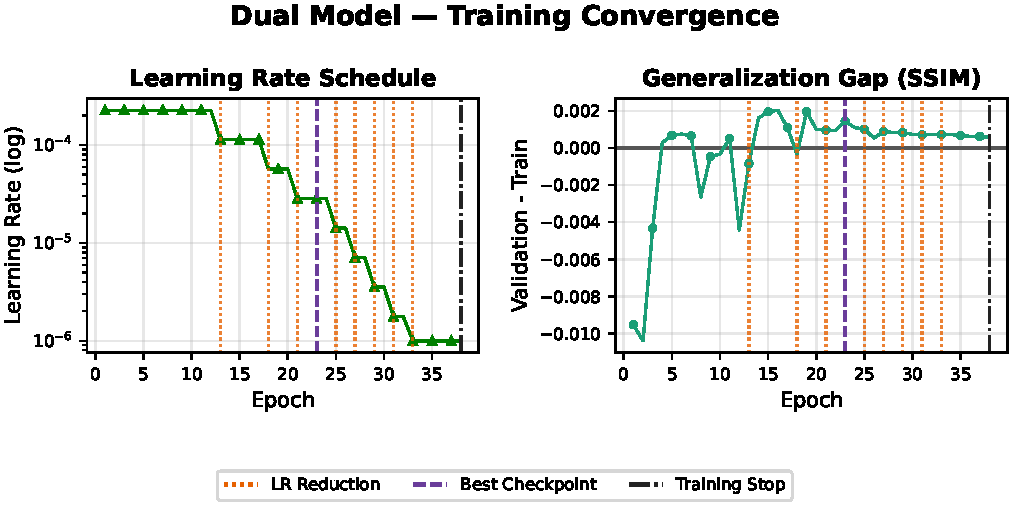
\includegraphics[width=0.98\linewidth]{Figures/Generated/training/training-curves-dualhead-pair-04-lr-gap-06e153c6.pdf}
\end{figure}

\FloatBarrier
\captionsetup{skip=1.5pt}
\graphiccaptionof[Training convergence (results): Dual Model, seed 2024]{Training convergence for the Dual Model, seed 2024. Each chart pair repeats the shared legend so it remains interpretable if the group spans multiple pages. Orange dotted vertical lines indicate learning-rate reductions; the purple dashed line marks the epoch of the best validation checkpoint; and the black dash-dotted line marks training termination. The \textit{generalization-gap} panel reports validation minus training SSIM and supports inspection for persistent divergence compatible with overfitting.}
\label{fig:results-training-convergence-dual-model-seed-2024}
\par\medskip
\endgroup

